\let\negmedspace\undefined{}
\let\negthickspace\undefined{}
\documentclass[journal,12pt,twocolumn]{IEEEtran}
 \usepackage{gensymb}
 \usepackage{polynom}
\usepackage{amssymb}
\usepackage[cmex10]{amsmath}
\usepackage{amsthm}
 \usepackage{stfloats}
\usepackage{bm} 
 \usepackage{longtable}
 \usepackage{enumitem}
 \usepackage{mathtools}
 \usepackage{tikz}
 \usepackage[breaklinks=true]{hyperref}
\usepackage{listings}
\usepackage{color}                                            
\usepackage{array}                                            
\usepackage{longtable}                                        
\usepackage{calc}                                             
    \usepackage{multirow}                                         
    \usepackage{hhline}                                           
    \usepackage{ifthen}                                           
    \usepackage{lscape} 
\DeclareMathOperator\erf{erf}    
\DeclareMathOperator*{\Res}{Res}
\DeclareMathOperator*{\equals}{=}
\renewcommand\thesection{\arabic{section}}
\renewcommand\thesubsection{\thesection.\arabic{subsection}}
\renewcommand\thesubsubsection{\thesubsection.\arabic{subsubsection}}
\renewcommand\thesectiondis{\arabic{section}}
\renewcommand\thesubsectiondis{\thesectiondis.\arabic{subsection}}
\renewcommand\thesubsubsectiondis{\thesubsectiondis.\arabic{subsubsection}}
\hyphenation{op-tical net-works semi-conduc-tor}
\def\inputGnumericTable{}                                 %%
\lstset{ 
frame=single,
breaklines=true,
columns=fullflexible
}
\begin{document}
\newtheorem{theorem}{Theorem}[section]
\newtheorem{problem}{Problem}
\newtheorem{proposition}{Proposition}[section]
\newtheorem{lemma}{Lemma}[section]
\newtheorem{corollary}[theorem]{Corollary}
\newtheorem{example}{Example}[section]
\newtheorem{definition}[problem]{Definition}
\newcommand{\BEQA}{\begin{eqnarray}}
\newcommand{\EEQA}{\end{eqnarray}}
\newcommand{\define}{\stackrel{\triangle}{=}}
\newcommand*\circled[1]{\tikz[baseline= (char.base)]{
    \node[shape=circle,draw,inner sep=2pt] (char) {#1};}}
\bibliographystyle{IEEEtran}
\providecommand{\mbf}{\mathbf}
\providecommand{\mygtrless}{
  \mathrel{
  \smash{
  \vcenter{
    \offinterlineskip{}
    \ialign{
       \hfil##\hfil\cr % just one centered column
       $0$\cr 
       \noalign{\kern-.3ex}
       $>$\cr 
       \noalign{\kern-.3ex}
       $<$\cr 
       \noalign{\kern-.3ex}
       $1$\cr 
    }% end of the \ialign
  }% end of \vcenter
  }% end of \smash
  \vphantom{>}% pretend it's as high as a >
  }% end of \mathrel
}
\providecommand{\gauss}[2]{\mathcal{N}\ensuremath{\left(#1,#2\right)}}
\providecommand{\pr}[1]{\ensuremath{\Pr\left(#1\right)}}
\providecommand{\qfunc}[1]{\ensuremath{Q\left(#1\right)}}
\providecommand{\sbrak}[1]{\ensuremath{{}\left[#1\right]}}
\providecommand{\lsbrak}[1]{\ensuremath{{}\left[#1\right.]}}
\providecommand{\rsbrak}[1]{\ensuremath{{}\left[#1\right.]}}
\providecommand{\brak}[1]{\ensuremath{\left(#1\right)}}
\providecommand{\lbrak}[1]{\ensuremath{\left(#1\right.)}
\providecommand{\rbrak}[1]{\ensuremath{\left[#1\right.]}}}
\providecommand{\cbrak}[1]{\ensuremath{\left\{#1\right\}}}
\providecommand{\lcbrak}[1]{\ensuremath{\left\{#1\right.}}
\providecommand{\rcbrak}[1]{\ensuremath{\left.#1\right\}}}
\providecommand{\ztrans}{\overset{\mathcal{Z}}{ \rightleftharpoons}}
\theoremstyle{remark}
\newtheorem{rem}{Remark}
\newcommand{\sgn}{\mathop{\mathrm{sgn}}}
\providecommand{\abs}[1]{\left\vert#1\right\vert}
\providecommand{\res}[1]{\Res\displaylimits_{#1}} 
\providecommand{\norm}[1]{\left\lVert#1\right\rVert}
\providecommand{\mtx}[1]{\mathbf{#1}}
\providecommand{\mean}[1]{E\left[ #1 \right]}
\providecommand{\fourier}{\overset{\mathcal{F}}{ \rightleftharpoons}}
\providecommand{\system}{\overset{\mathcal{H}}{ \longleftrightarrow}}
\newcommand{\solution}{\noindent \textbf{Solution: }}
\newcommand{\cosec}{\,\text{cosec}\,}
\newcommand*{\permcomb}[4][0mu]{{{}^{#3}\mkern#1#2_{#4}}}
\newcommand*{\perm}[1][-3mu]{\permcomb[#1]{P}}
\newcommand*{\comb}[1][-1mu]{\permcomb[#1]{C}}
\renewcommand{\thetable}{\arabic{table}} 
\providecommand{\dec}[2]{\ensuremath{\overset{#1}{\underset{#2}{\gtrless}}}}
\newcommand{\myvec}[1]{\ensuremath{\begin{pmatrix}#1\end{pmatrix}}}
\newcommand{\mydet}[1]{\ensuremath{\begin{vmatrix}#1\end{vmatrix}}}
\numberwithin{equation}{section}
\numberwithin{figure}{section}
\numberwithin{table}{section} 
\makeatletter
\@addtoreset{figure}{problem} 
\makeatother
\let\StandardTheFigure\thefigure{} 
\let\vec\mathbf{}
\def\putbox#1#2#3{\makebox[0in][l]{\makebox[#1][l]{}\raisebox{\baselineskip}[0in][0in]{\raisebox{#2}[0in][0in]{#3}}}}
     \def\rightbox#1{\makebox[0in][r]{#1}}
     \def\centbox#1{\makebox[0in]{#1}}
     \def\topbox#1{\raisebox{-\baselineskip}[0in][0in]{#1}}
     \def\midbox#1{\raisebox{-0.5\baselineskip}[0in][0in]{#1}}
\vspace{3cm}
\title{Digital Signal Processing}
\author{Gunjit Mittal (AI21BTECH11011)}
\maketitle
\tableofcontents 
\renewcommand{\thefigure}{\theenumi}
\renewcommand{\thetable}{\theenumi}
%\renewcommand{\theequation}{\thesection}
\bigskip
\begin{abstract}
This manual provides a simple introduction to digital signal processing.
\end{abstract}
\section{Software Installation}
Run the following commands
\begin{lstlisting}
sudo apt-get update
sudo apt-get install libffi-dev libsndfile1 python3-scipy  python3-numpy python3-matplotlib 
sudo pip install cffi pysoundfile 
\end{lstlisting}
\section{Digital Filter}
\begin{enumerate}[label=\thesection.\arabic*
,ref=\thesection.\theenumi]
\item
\label{prob:input}
Download the sound file from  
\begin{lstlisting}
wget https://github.com/gunjitmittal/EE3900/blob/main/Assignment-1/codes/Sound_Noise.wav
\end{lstlisting}
%\href{http://tlc.iith.ac.in/img/sound/Sound_Noise.wav}{\url{http://tlc.iith.ac.in/img/sound/Sound_Noise.wav}}  
%in the link given below.
%\linebreak
\item
\label{prob:spectrogram}
You will find a spectrogram at \href{https://academo.org/demos/spectrum-analyzer}{\url{https://academo.org/demos/spectrum-analyzer}}. 
%\end{problem}
%%
%
%%\onecolumn
%%\input{./figs/fir}
%\begin{problem}
Upload the sound file that you downloaded in Problem \ref{prob:input} in the spectrogram  and play.  Observe the spectrogram. What do you find?
\\
%
\solution 
By observing spectrogram, it clearly shows that tonal frequency is under 4kHz. And above 4kHz only noise is present.
\item \label{prob:output}
Write the python code for removal of out of band noise and execute the code.
\\
\solution
\lstinputlisting{./codes/noise_rm.py}
\item
The output of the python script in Problem \ref{prob:output} is the audio file Sound\_With\_ReducedNoise.wav. Play the file in the spectrogram in Problem \ref{prob:spectrogram}. What do you observe?
\\
\solution The audio is subdued and the higher frequenices are just blank.
\end{enumerate}
\section{Difference Equation}
\begin{enumerate}[label=\thesection.\arabic*,ref=\thesection.\theenumi]
\item Let
\label{def:xn}
\begin{equation}
x(n) = \cbrak{\underset{\uparrow}{1},2,3,4,2,1}
\end{equation}
Sketch $x(n)$.
\item Let
\begin{multline}
\label{eq:iir_filter}
y(n) + \frac{1}{2}y(n-1) = x(n) + x(n-2), 
\\
 y(n) = 0, n < 0
\end{multline}
Sketch $y(n)$.
\\
\solution The following code yields Fig. \ref{fig:xnyn}.
\begin{lstlisting}
wget https://github.com/gunjitmittal/EE3900/blob/main/Assignment-1/codes/xnyn.py
\end{lstlisting}
\begin{figure}[!ht]
\begin{center}
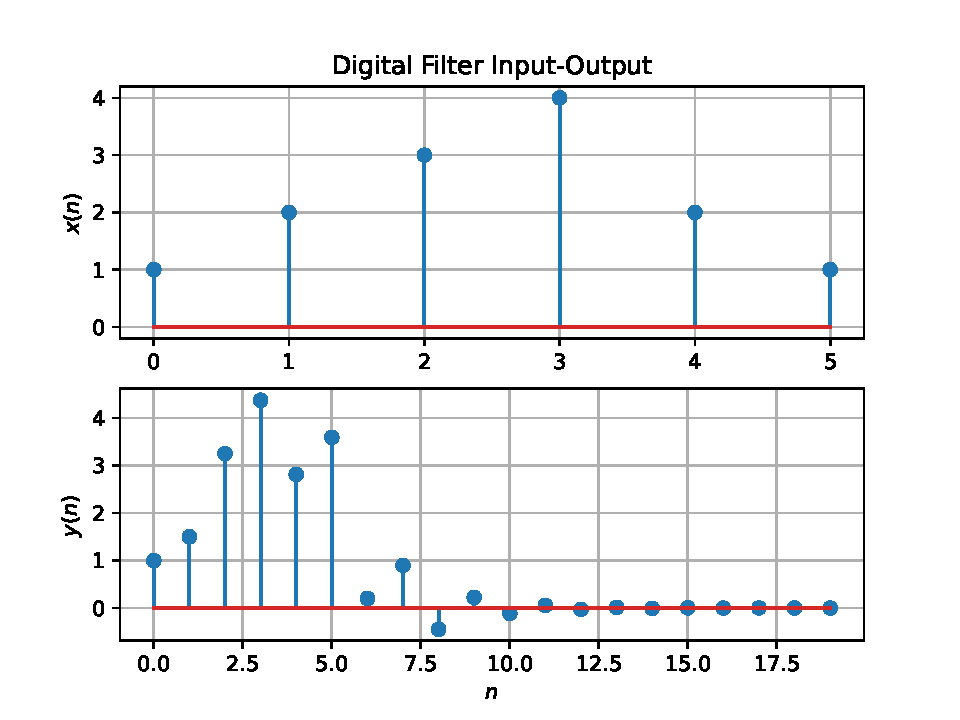
\includegraphics[width=\columnwidth]{./figs/xnyn}
\end{center}
\caption{figure}{}
\label{fig:xnyn}	
\end{figure}
\item Repeat the above exercise using a C code.
\solution
Download and run the C code for generating y and Python code for plotting y
\begin{lstlisting}
  wget https://github.com/gunjitmittal/EE3900/blob/main/Assignment-1/codes/xnyn.c
  wget https://github.com/gunjitmittal/EE3900/blob/main/Assignment-1/codes/xnyn(1).py
  \end{lstlisting}
  \begin{figure}[!ht]
    \begin{center}
    \includegraphics[width=\columnwidth]{./figs/xnyn(1)}
    \end{center}
    \caption{figure}{}
    \label{fig:xnyn(1)}	
    \end{figure}
\end{enumerate}
\section{$Z$-transform}
\begin{enumerate}[label=\thesection.\arabic*]
\item The $Z$-transform of $x(n)$ is defined as
%
\begin{equation}
\label{eq:z_trans}
X(z)={\mathcal {Z}}\{x(n)\}=\sum _{n=-\infty }^{\infty }x(n)z^{-n}
\end{equation}
%
Show that
\begin{equation}
\label{eq:shift1}
{\mathcal {Z}}\{x(n-1)\} = z^{-1}X(z)
\end{equation}
and find
\begin{equation}
	{\mathcal {Z}}\{x(n-k)\} 
\end{equation}
\solution From \eqref{eq:z_trans},
\begin{align}
{\mathcal {Z}}\{x(n-1)\} &=\sum _{n=-\infty }^{\infty }x(n-1)z^{-n}
\\
&=\sum _{n=-\infty }^{\infty }x(n)z^{-n-1} \\
&=z^{-1}\sum _{n=-\infty }^{\infty }x(n)z^{-n}
\end{align}
resulting in \eqref{eq:shift1}. Similarly, it can be shown that
%
\begin{align}
  {\mathcal {Z}}\{x(n-k)\} &=\sum _{n=-\infty }^{\infty }x(n-k)z^{-n}
  \\
  &=\sum _{n=-\infty }^{\infty }x(n)z^{-n-k} \\
  &=z^{-k}\sum _{n=-\infty }^{\infty }x(n)z^{-n}
  \label{eq:z_trans_shift}
  \end{align}
\item Obtain $X(z)$ for $x(n)$ defined in problem 
	\ref{def:xn}.
\solution \\
\begin{align}
  X(z)&=\sum _{n=0}^{5}x(n)z^{-n}\\
  &= 1 + 2z^{-1} + 3z^{-2} + 4z^{-3} + 2z^{-4} + 1z^{-5}
\end{align}
\item Find
%
\begin{equation}
H(z) = \frac{Y(z)}{X(z)}
\end{equation}
%
from  \eqref{eq:iir_filter} assuming that the $Z$-transform is a linear operation.
\\
\solution We have
\begin{align}
  y(n) + \frac{1}{2}y(n-1) = x(n) + x(n-2)
\end{align} 
Finding the Z-transform 
\begin{align}
  {\mathcal {Z}}\{y(n) + \frac{1}{2}y(n-1)\} &= {\mathcal {Z}}\{x(n)+x(n-2)\}
\end{align}
Because Z-transform is a linear function
\begin{align}
  {\mathcal {Z}}y(n) + \frac{1}{2}{\mathcal {Z}}y(n-1) &= {\mathcal {Z}}x(n)+{\mathcal {Z}}x(n-2)
\end{align}
Using \eqref{eq:z_trans_shift}
\begin{align}
  Y(z) + \frac{1}{2}z^{-1}Y(z) &= X(z)+z^{-2}X(z)
\end{align}
\begin{align}
\implies \frac{Y(z)}{X(z)} &= \frac{1 + z^{-2}}{1 + \frac{1}{2}z^{-1}}
\label{eq:freq_resp}
\end{align}
\item Find the Z transform of 
\begin{equation}
\delta(n)
=
\begin{cases}
1 & n = 0
\\
0 & \text{otherwise}
\end{cases}
\end{equation}
and show that the $Z$-transform of
\begin{equation}
\label{eq:unit_step}
u(n)
=
\begin{cases}
1 & n \ge 0
\\
0 & \text{otherwise}
\end{cases}
\end{equation}
is
\begin{equation}
U(z) = \frac{1}{1-z^{-1}}, \quad \abs{z} > 1
\end{equation}
\solution 
\begin{align}
\delta(n) &\ztrans \sum _{n=-\infty }^{\infty }\delta(n)z^{-n}\\
&= \sum _{n=0}z^{-n} = 1
\end{align}
and from \eqref{eq:unit_step},
\begin{align}
u(n) &\ztrans U(z) = \sum _{n=-\infty }^{\infty }u(n)z^{-n}\\
U(z) &= \sum _{n= 0}^{\infty}z^{-n}\\
&=\frac{1}{1-z^{-1}}, \quad \abs{z} > 1
\end{align}
using the fomula for the sum of an infinite geometric progression.
%
\item Show that 
\begin{equation}
\label{eq:anun}
a^nu(n) \ztrans \frac{1}{1-az^{-1}} \quad \abs{z} > \abs{a}
\end{equation}
\solution
\begin{align}
  a^nu(n) &\ztrans \sum _{n=-\infty }^{\infty }a^n u(n)z^{-n}\\
  &= \sum _{n=0 }^{\infty } (az^{-1})^{-n}\\
  &=\frac{1}{1-az^{-1}}, \quad \abs{z} > \abs{a}
\end{align}
\item 
Let
\begin{equation}
H\brak{e^{\j \omega}} = H\brak{z = e^{\j \omega}}.
\end{equation}
Plot $\abs{H\brak{e^{\j \omega}}}$.  Comment.  $H(e^{\j \omega})$ is
known as the {\em Discret Time Fourier Transform} (DTFT) of $h(n)$.
\\
\solution
\begin{align}
  H\brak{e^{\j \omega}} &= \frac{1 + e^{-2\j\omega}}{1 + \frac12 e^{-\j\omega}} \\
  \implies \abs{H\brak{e^{\j \omega}}} &= \frac{\abs{1 + \cos2\omega - \j\sin2\omega}}{\abs{1 + \frac12 \cos\omega - \frac12 \sin\omega}} \\
  &= \sqrt{\frac{(1 + \cos2\omega)^2 + (\sin2\omega)^2}{(1 + \frac12 \cos\omega)^2 + (\frac12 \sin\omega)^2}} \\
  &= \sqrt{\frac{2 + 2\cos2\omega}{\frac54 + \cos\omega}} \\
  &= \sqrt{\frac{2(2\cos^2\omega)4}{5 + 4\cos\omega} } \\
  &= \frac{4\abs{\cos\omega}}{\sqrt{5 + 4\cos\omega}}
\end{align}
 The following code plots Fig. \ref{fig:dtft}.
\begin{lstlisting}
wget https://github.com/gunjitmittal/EE3900/blob/main/Assignment-1/codes/dtft.py
\end{lstlisting}
The plot is even and has a period of $2\pi $.
% The plot achieves it's global maxima at $\pm(2n+1)\pi$ and global minima at $\pm 2n\pi$
\begin{figure}[!ht]
\centering
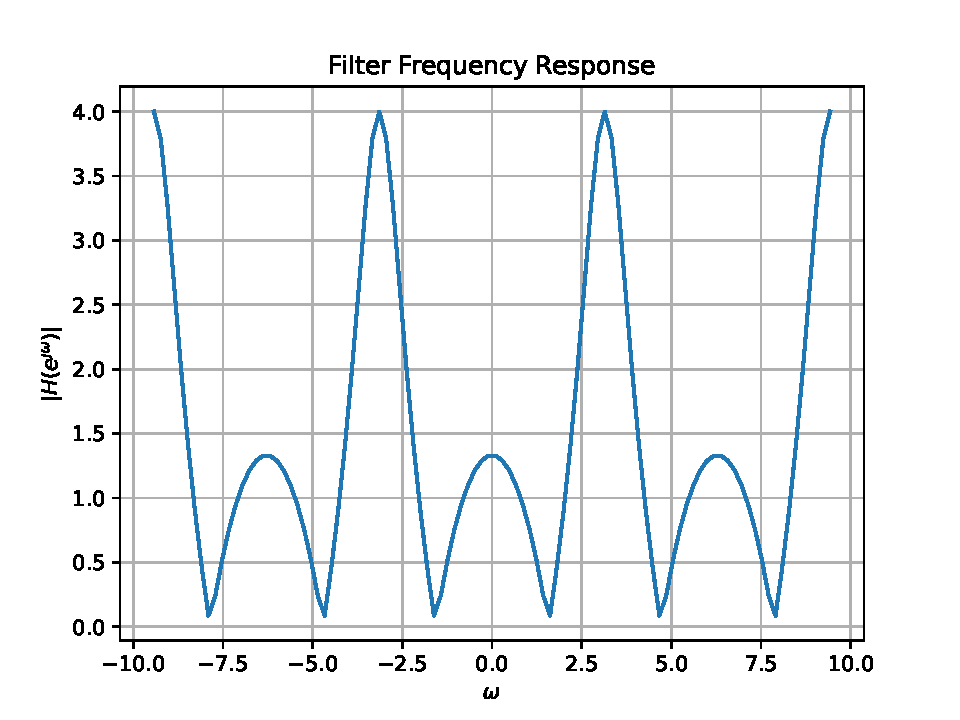
\includegraphics[width=\columnwidth]{./figs/dtft}
\caption{$\abs{H\brak{e^{j\omega}}}$}
\label{fig:dtft}
\end{figure}
\item Express $h(n)$ in terms of $H\brak{e^{j \omega}}$.\\
\solution Since $H\brak{e^{j \omega}}$ is the DTFT of $h(n)$
\begin{align}
  &\int_{-\pi}^{\pi} H\brak{e^{j\omega}} e^{jn\omega} d\omega\\
  &=\int_{-\pi}^{\pi} \brak{\sum_{k=-\infty}^{\infty} h(k) e^{-jk\omega}} e^{jn\omega} d\omega\\
  &=\sum_{k=-\infty}^{\infty} h(k) \int_{-\pi}^{\pi}  e^{j(n-k)\omega} d\omega\\
  &=2\pi \sum_{k=-\infty}^{\infty} h(k) \delta(n-k)\\
  &=2\pi h(n)
\end{align}
\begin{equation}
  \therefore h(n) = \frac{1}{2\pi} \int_{-\pi}^{\pi} H\brak{e^{j\omega}} e^{jn\omega} d\omega
\end{equation}
\end{enumerate}
\section{Impulse Response}
\begin{enumerate}[label=\thesection.\arabic*]
  \item Using long division, find
	\begin{align}
		h(n), \quad n < 5
	\end{align}
	for $H(z)$ in \eqref{eq:freq_resp}
	
	\solution 
  \begin{equation}
		H(z) = \frac{1 + z^{-2}}{1 + \frac12 z^{-1}}
	\end{equation}
	Substitute $z^{-1} = x$
	
	\polylongdiv{1+x^2}{1+\frac12 x}
	
	\begin{align}
		&\implies 1 + z^{-2} = \brak{1 + \frac12 z^{-1}}\brak{-4 + 2z^{-1}} + 5 \\
		&\implies H(z) = -4 + 2z^{-1} + \frac{5}{1 + \frac12 z^{-1}}
	\end{align}
	
	On applying the inverse $Z$-transform on both sides of the equation
	\begin{align}
		H(z) &\ztrans h(n) \\
		-4 &\ztrans -4\delta(n) \\
		2z^{-1} &\ztrans 2\delta(n - 1) \\
		\frac{5}{1 + \frac12 z^{-1}} &\ztrans 5\brak{-\frac12}^n u(n) \\
	\end{align}
	
	Therefore,
	\begin{equation}
		h(n) = -4\delta(n) + 2\delta(n - 1) + 5\brak{-\frac12}^n u(n)
	\end{equation}
  \begin{align}
    &h(0) = -4 + 5 = 1\\
    &h(1) = 2 - 2.5 = -0.5\\
    &h(2) = 1.25\\
    &h(3) = -0.625\\
    &h(4) = 0.3125
  \end{align}
\item \label{prob:impulse_resp}
Find an expression for $h(n)$ using $H(z)$, given that 
%in Problem \ref{eq:ztransab} and \eqref{eq:anun}, given that
\begin{equation}
\label{eq:impulse_resp}
h(n) \ztrans H(z)
\end{equation}
and there is a one to one relationship between $h(n)$ and $H(z)$. $h(n)$ is known as the {\em impulse response} of the
system defined by \eqref{eq:iir_filter}.
\\
\solution From \eqref{eq:freq_resp},
\begin{align}
H(z) &= \frac{1}{1 + \frac{1}{2}z^{-1}} + \frac{ z^{-2}}{1 + \frac{1}{2}z^{-1}}
\\
\implies h(n) &= \brak{-\frac{1}{2}}^{n}u(n) + \brak{-\frac{1}{2}}^{n-2}u(n-2)
\end{align}
using \eqref{eq:anun} and \eqref{eq:z_trans_shift}.
\item Sketch $h(n)$. Is it bounded? Justify theoretically.
\\
\solution The following code plots Fig. \ref{fig:hn}.
\begin{lstlisting}
wget https://github.com/gunjitmittal/EE3900/blob/main/Assignment-1/codes/hn.py
\end{lstlisting}
\begin{figure}[!ht]
\centering
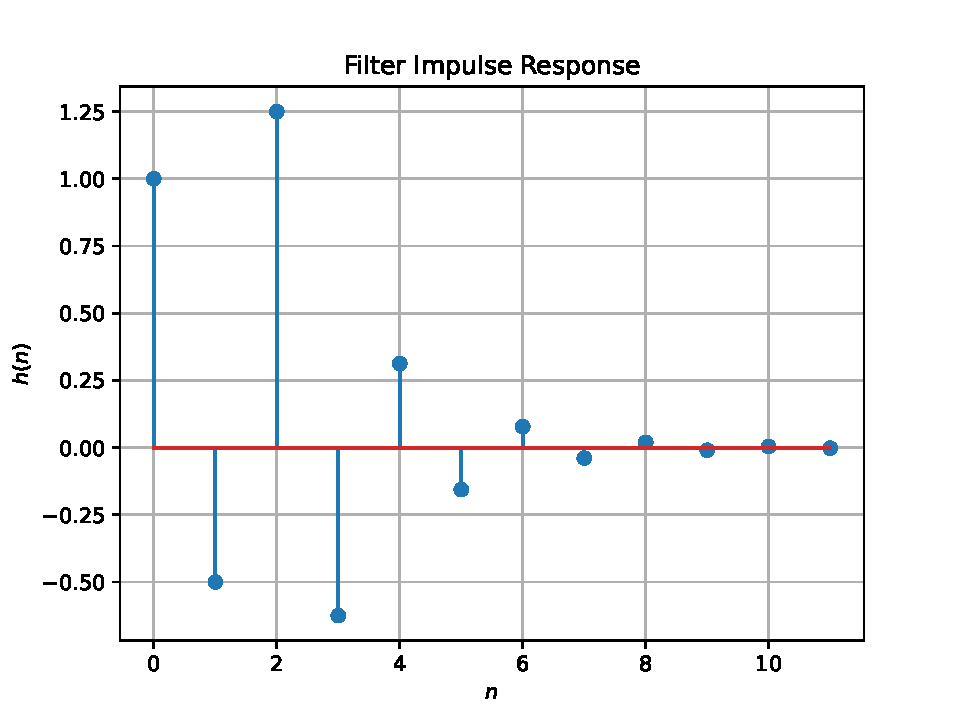
\includegraphics[width=\columnwidth]{./figs/hn}
\caption{$h(n)$ as the inverse of $H(z)$}
\label{fig:hn}
\end{figure}
As we can see from the plot $h(n)$ is bounded.
Theoretically,
	\begin{align}
		&\abs{u(n)} &\le 1 \\
		&\abs{\brak{-\frac12}^n} &\le 1 \\
		\implies &\abs{\brak{-\frac12}^n u(n)} &\le 1
	\end{align}
	
	Similarly,
	\begin{align}
		&\abs{\brak{-\frac12}^{n-2} u(n-2)} &\le 1 \\
		\implies &h(n) &\le 2
	\end{align}
	
	Therefore $h(n)$ is bounded.
  \item Is it convergetn? Justify using ratio test.\\
  \solution Using the ratio test for convergence
	\begin{align}
		\lim_{n \to \infty} \abs{\frac{h(n+1)}{h(n)}} &= \lim_{n \to \infty} \abs{\frac{\brak{-\frac12}^{n-1} \brak{\frac14 + 1}}{\brak{-\frac12}^{n-2} \brak{\frac14 + 1}}} \\
		&= \lim_{n \to \infty} \abs{-\frac12} \\
		&= \frac{1}{2} < 1
	\end{align}
	
	Therefore, $h(n)$ is convergent.
\item The system with $h(n)$ is defined to be stable if
\begin{equation}
\sum_{n=-\infty}^{\infty}h(n) < \infty
\end{equation}
Is the system defined by \eqref{eq:iir_filter} stable for the impulse response in \eqref{eq:impulse_resp}?\\
\solution
	\begin{multline}
		\sum_{n=-\infty}^{\infty}h(n) = \sum_{n=-\infty}^{\infty} \brak{-\frac12}^n u(n) \\
		+ \sum_{n=-\infty}^{\infty} \brak{-\frac12}^{n-2} u(n-2)
	\end{multline}
	\begin{align}
		\sum_{n=-\infty}^{\infty}h(n) = \sum_{n=0}^{\infty}\brak{-\frac12}^n + \sum_{n=2}^{\infty}\brak{-\frac12}^{n-2}
	\end{align}
	
	These are both sums of infinite geometric progressions with first terms $1$ and common ratios $-\frac12$
	\begin{align}
		\sum_{n=-\infty}^{\infty}h(n) &= \frac{1}{1 - \brak{-\frac12}} + \frac{1}{1 - \brak{-\frac12}} \\
		&= \frac{4}{3} < \infty
	\end{align}
	Therefore, the system is stable. 
  \item Verify the above result using a Python code. 
	
	\solution The stability has been verified in the following code
  \begin{lstlisting}
    wget https://github.com/gunjitmittal/EE3900/blob/main/Assignment-1/codes/hndef.py
    \end{lstlisting}
\item 
Compute and sketch $h(n)$ using 
\begin{equation}
\label{eq:iir_filter_h}
h(n) + \frac{1}{2}h(n-1) = \delta(n) + \delta(n-2), 
\end{equation}
%
This is the definition of $h(n)$.
\\
\solution 
	\begin{equation}
		h(0) = 1
	\end{equation}
	
	Now, for $n = 1$,
	\begin{align}
		h(1) + \frac12 h(0) &= \delta(1) + \delta(-1) = 0 \\
		\implies h(1) &= - \frac{1}{2} h(0) = -\frac{1}{2}
	\end{align}
	
	For $n = 2$,
	\begin{align}
		h(2) + \frac12 h(1) &= \delta(2) + \delta(0) = 1 \\
		\implies h(2) &= 1 - \frac{1}{2} h(1) = \frac{5}{4}
	\end{align}
	
	For $n > 2$, the right hand side of the equation is always zero. Thus,
	\begin{align}
		h(n) &= -\frac{1}{2} h(n-1) \qquad n > 2 \\
		h(3) &= \frac{5}{4} \brak{-\frac12} \\
		h(4) &= \frac{5}{4} \brak{-\frac12}^2 \\
		&~\vdots \\
		h(n) &= \frac{5}{4} \brak{-\frac12}^{n-2}
	\end{align}
	
	Therefore,
	\begin{align}
		h(n) = 
		\begin{cases}
			1 & n = 0 \\
			-\dfrac{1}{2} & n = 1 \\
			\dfrac{5}{4} \brak{-\dfrac12}^{n-2} & n \ge 2
		\end{cases}
	\end{align}
	
	Thus, it is bounded and convergent to $0$
	\begin{equation}
		\lim_{n \to \infty} h(n) = 0
	\end{equation}
   The following code plots Fig. \ref{fig:hndef}. Note that this is the same as Fig. 
\ref{fig:hn}. 
\begin{lstlisting}
wget https://github.com/gunjitmittal/EE3900/blob/main/Assignment-1/codes/hndef.py
\end{lstlisting}
\begin{figure}[!ht]
\centering
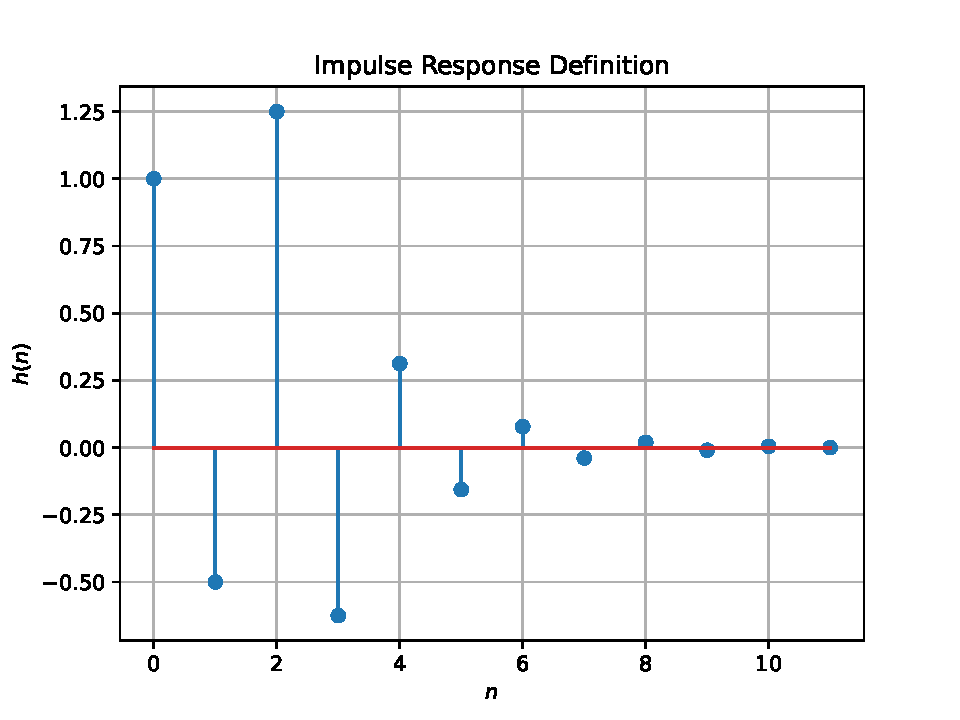
\includegraphics[width=\columnwidth]{./figs/hndef}
\caption{$h(n)$ from the definition}
\label{fig:hndef}
\end{figure}
%
\item Compute 
%
\begin{equation}
\label{eq:convolution}
y(n) = x(n)*h(n) = \sum_{k=-\infty}^{\infty}x(k)h(n-k)
\end{equation}
%
Comment. The operation in \eqref{eq:convolution} is known as
{\em convolution}.
%
\\
\solution The following code plots Fig. \ref{fig:ynconv}. Note that this is the same as 
$y(n)$ in  Fig. 
\ref{fig:xnyn}. 
%
\begin{lstlisting}
wget https://github.com/gunjitmittal/EE3900/blob/main/Assignment-1/codes/ynconv.py
\end{lstlisting}
\begin{figure}[!ht]
\centering
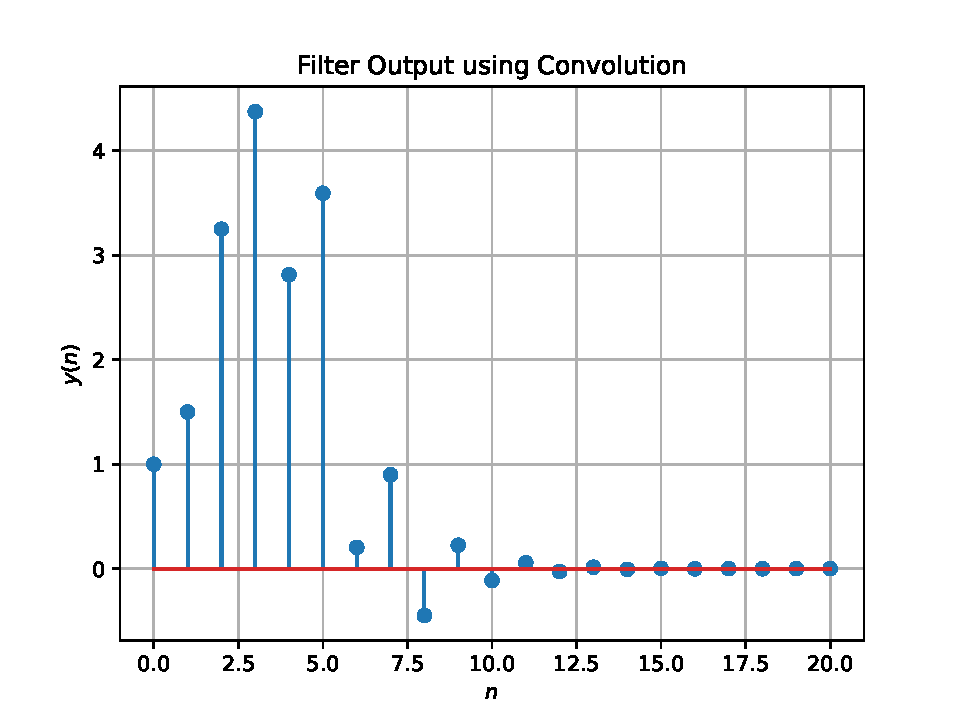
\includegraphics[width=\columnwidth]{./figs/ynconv}
\caption{$y(n)$ from the definition of convolution}
\label{fig:ynconv}
\end{figure}
\item Express the above convolution using a Toeplitz matrix.
	
	\solution Let 
	\begin{align}
		\vec{x} = \myvec{1 \\ 2 \\ 3 \\ 4 \\ 2 \\ 1} \qquad
		\vec{h} = \myvec{1 \\ -0.5 \\ 1.25 \\ -0.62 \\ 0.31 \\ -0.16}
	\end{align}
	
	Their convolution is given by the product of the following Toeplitz matrix $\vec{T}$
	\begin{align}
		\myvec{
			1 & 0 & 0 & 0 & 0 & 0 \\
			-0.5 & 1 & 0 & 0 & 0 & 0 \\
			1.25 & -0.5 & 1 & 0 & 0 & 0 \\
			-0.62 & 1.25 & -0.5 & 1 & 0 & 0 \\
			0.31 & -0.62 & 1.25 & -0.5 & 1 & 0 \\
			-0.16 & 0.31 & -0.62 & 1.25 & -0.5 & 1 \\
			0 & -0.16 & 0.31 & -0.62 & 1.25 & -0.5 \\
			0 & 0 & -0.16 & 0.31 & -0.62 & 1.25 \\
			0 & 0 & 0 & -0.16 & 0.31 & -0.62 \\
			0 & 0 & 0 & 0 & -0.16 & 0.31 \\
			0 & 0 & 0 & 0 & 0 & -0.16 \\
		} 
	\end{align}
	and $\vec{x}$
	
	\begin{align}
		&\vec{y} = \vec{x} \circledast \vec{h} = \vec{Tx} = \myvec{1 \\ 1.5 \\ 3.25 \\ 4.38 \\ 2.81 \\ 3.59 \\ 0.12 \\ 0.78 \\ -0.62 \\ 0 \\ -0.16}
	\end{align}
	
	Download the following Python code for computing the convolution by using a Toeplitz matrix and plotting Fig. \ref{fig-5.9}
	\begin{lstlisting}
		wget https://github.com/Ankit-Saha-2003/EE3900/raw/main/Assignment_1/codes/5.9.py
	\end{lstlisting}
	
	Run the Python code by executing
	\begin{lstlisting}
		python 5.9.py
	\end{lstlisting}

	\begin{figure}[!ht]
		\centering
		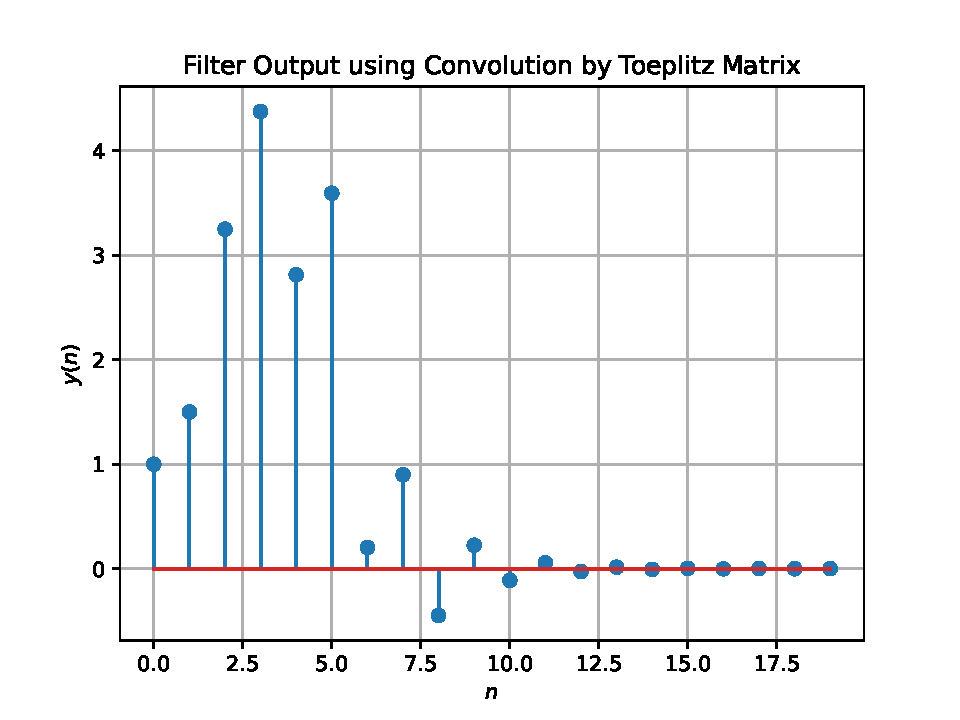
\includegraphics[width=\columnwidth]{./figs/5.9.pdf}
		\caption{Plot of the convolution of $x(n)$ and $h(n)$}
		\label{fig-5.9}	
	\end{figure}
\item Show that
\begin{equation}
y(n) =  \sum_{k=-\infty}^{\infty}x(n-k)h(k)
\end{equation}
\end{enumerate}
\solution
From \eqref{eq:convolution}
\begin{align}
  y(n) = \sum_{k=-\infty}^\infty x(k)h(n-k)
\end{align}
Substituting $k$ with $n-k$
\begin{align}
~~~~~~~~= \sum_{n-k=-\infty}^\infty x(n-k)h(k)
\end{align}
as $n$ remains constant, we can rewrite it as
\begin{align}
  ~~~~~~= \sum_{k=-\infty}^\infty x(n-k)h(k)
\end{align}
\section{DFT and FFT}
\begin{enumerate}[label=\thesection.\arabic*]
\item
Compute
\begin{equation}
X(k) \define \sum _{n=0}^{N-1}x(n) e^{-\j2\pi kn/N}, \quad k = 0,1,\dots, N-1
\end{equation}
and $H(k)$ using $h(n)$.\\
\solution 
\begin{figure}[!ht]
  \centering
  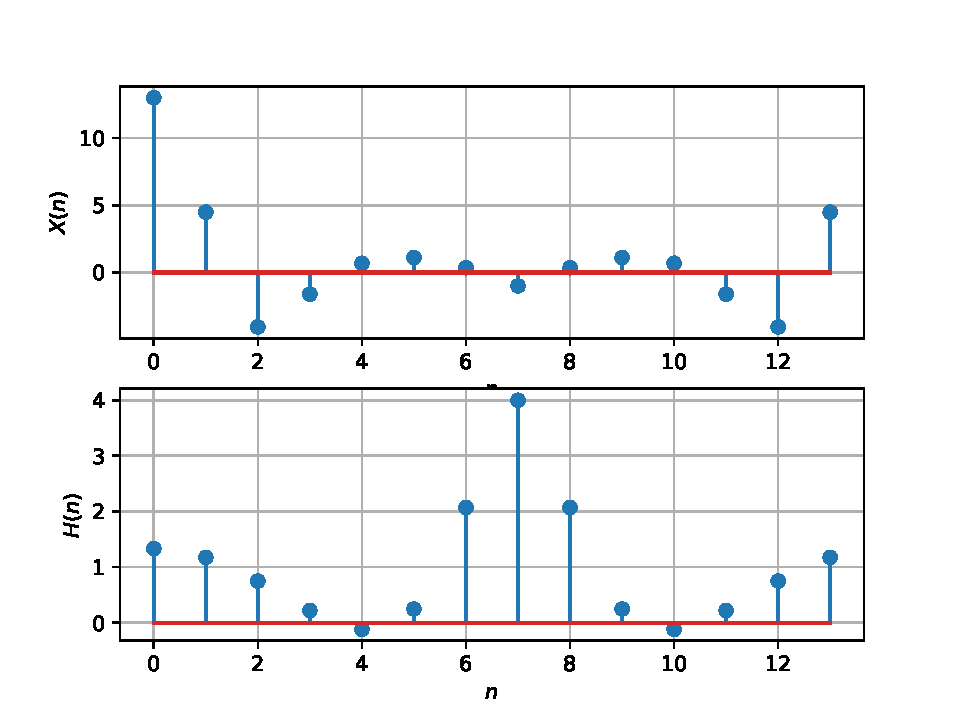
\includegraphics[width=\columnwidth]{./figs/X-H(n).pdf}
  \caption{$X(n) and H(n)$}
  \label{fig:X-H(n)}
  \end{figure}
  The following code plots Fig. \ref{fig:X-H(n)}.
%
\begin{lstlisting}
wget https://github.com/gunjitmittal/EE3900/blob/main/Assignment-1/codes/6_1.py
\end{lstlisting}
\item Compute 
\begin{equation}
Y(k) = X(k)H(k)
\label{eq:fp}
\end{equation}
\solution 
\begin{figure}[!ht]
  \centering
  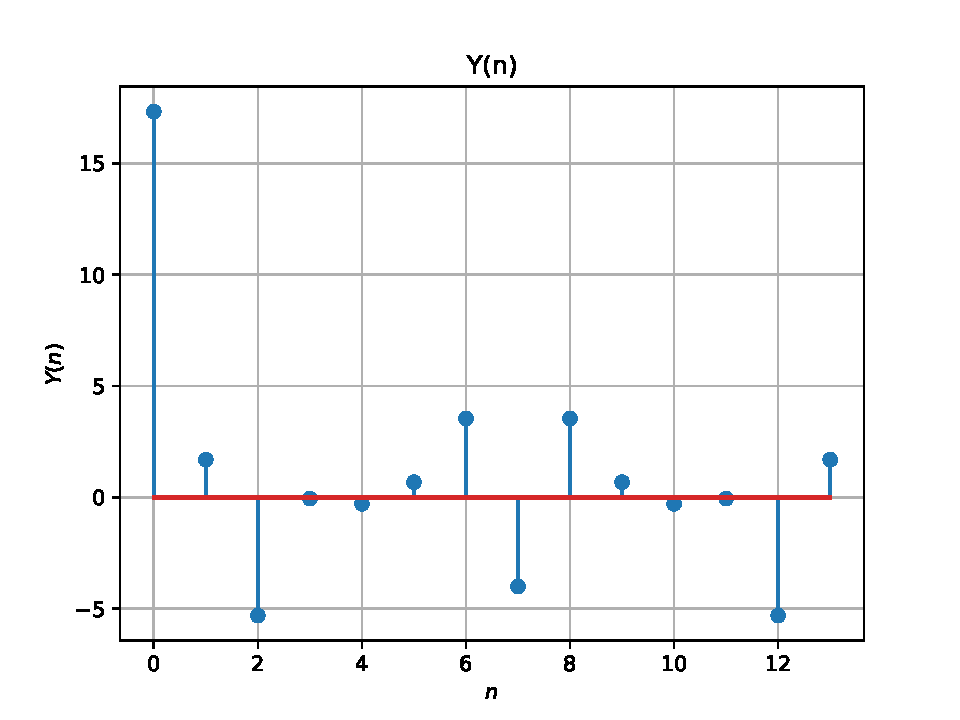
\includegraphics[width=\columnwidth]{./figs/Y(n).pdf}
  \caption{$Y(n)$}
  \label{fig:Y(n)}
  \end{figure}
  The following code plots Fig. \ref{fig:Y(n)}.
%
\begin{lstlisting}
wget https://github.com/gunjitmittal/EE3900/blob/main/Assignment-1/codes/6_2.py
\end{lstlisting}
\item Compute
\begin{equation}
  y\brak{n}={\frac {1}{N}}\sum _{k=0}^{N-1}Y\brak{k}\cdot e^{\j 2\pi kn/N},\quad n = 0,1,\dots, N-1
  \label{eq:inv-ft}
 \end{equation}
 \\
 \solution The following code plots Fig. \ref{fig:ynconv}. Note that this is the same as 
 $y(n)$ in  Fig. 
 \ref{fig:xnyn}. 
 %
 \begin{lstlisting}
 wget https://github.com/gunjitmittal/EE3900/blob/main/Assignment-1/codes/yndft.py
 \end{lstlisting}
 \begin{figure}[!ht]
 \centering
 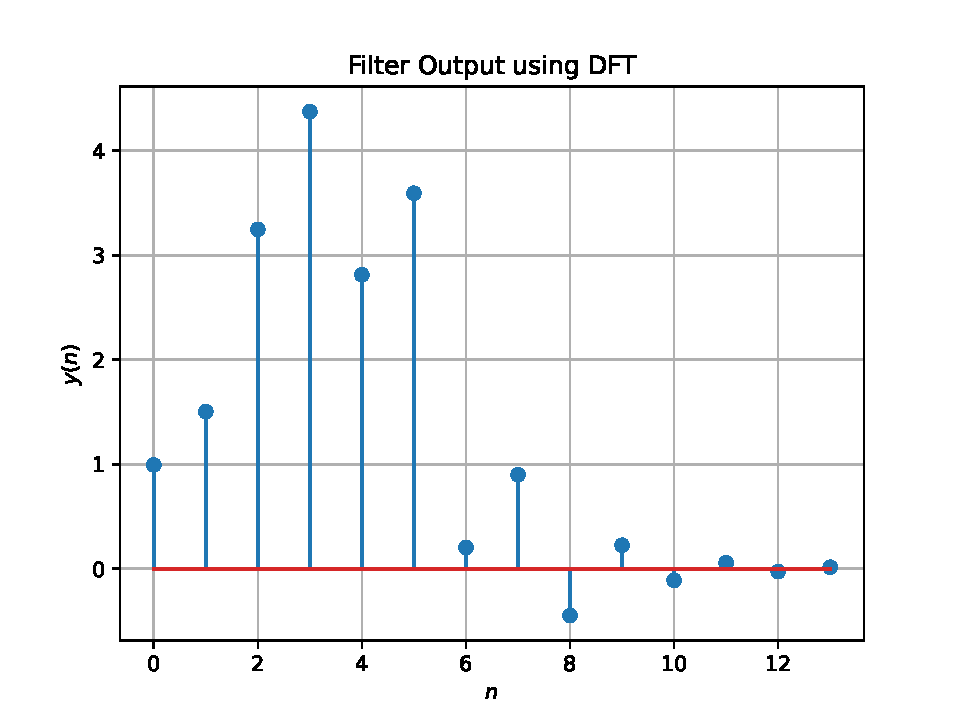
\includegraphics[width=\columnwidth]{./figs/yndft}
 \caption{$y(n)$ from the DFT}
 \label{fig:yndft}
 \end{figure}
 \item Repeat the previous exercise by computing $X(k), H(k)$ and $y(n)$ through FFT and 
 IFFT.\\
 \solution
 \begin{figure}[!ht]
  \centering
  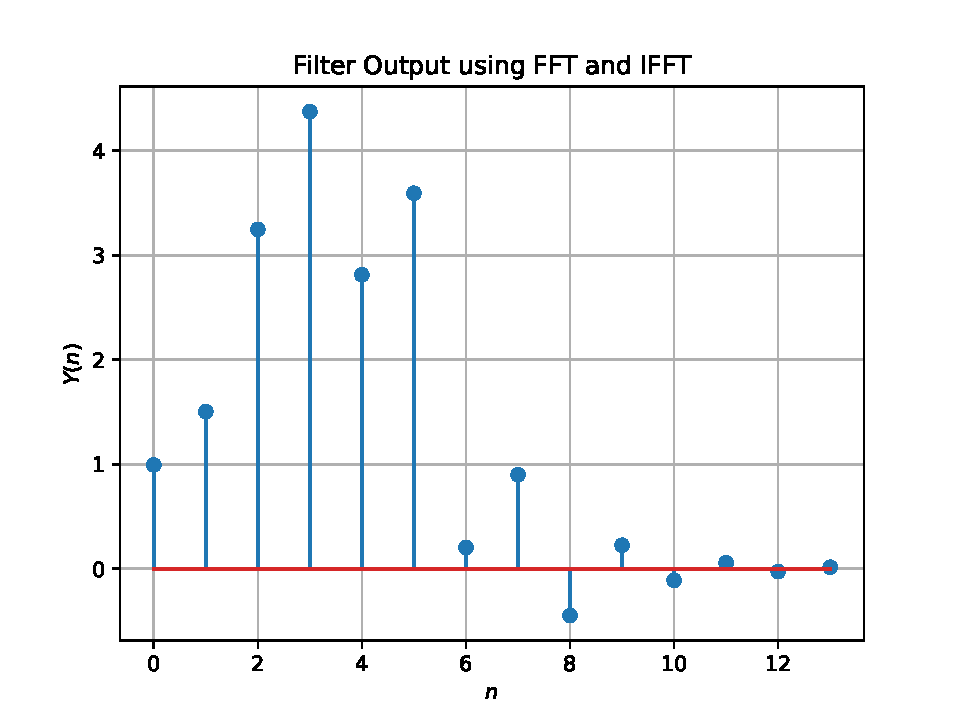
\includegraphics[width=\columnwidth]{./figs/6_4.pdf}
  \caption{$y(n)$ using FFT and IFFT}
  \label{fig:y(n)_FFT}
  \end{figure}
  The following code plots Fig. \ref{fig:y(n)_FFT}.
%
\begin{lstlisting}
wget https://github.com/gunjitmittal/EE3900/blob/main/Assignment-1/codes/6_4.py
\end{lstlisting}
 \item Wherever possible, express all the above equations as matrix equations.\\
 \solution
 We use the DFT Matrix, where $\omega = e^{-\frac{j2k\pi}{N}}$, which is given by
 \begin{align}
   \mtx{W} = 
   \begin{pmatrix}
     \omega^0 & \omega^0 & \ldots & \omega^0 \\
     \omega^0 & \omega^1 & \ldots & \omega^{N - 1} \\
     \vdots & \vdots & \ddots & \vdots \\
     \omega^0 & \omega^{N - 1} & \ldots & \omega^{(N -1)(N - 1)}
   \end{pmatrix}
 \end{align}
 i.e. $W_{jk} = \omega^{jk}$, $0 \leq j, k < N$. Hence, we can write any DFT equation as
 \begin{align}
   \mtx{X} = \mtx{W}\mtx{x} = \mtx{x}\mtx{W}
 \end{align}
 \noindent where
 \begin{align}
   \mtx{x} = 
   \begin{pmatrix}
     x(0) \\ x(1) \\ \vdots \\ x(n - 1)
   \end{pmatrix}
 \end{align}
 \noindent Using \eqref{eq:inv-ft}, the inverse Fourier Transform is given by
 \begin{align}
   \mtx{x} = \mathcal{F}^{-1}\brak{\mtx{X}} = \mtx{W}^{-1}\mtx{X} &= \frac{1}{N}\mtx{W^{H}}\mtx{X} = \frac{1}{N}\mtx{X}\mtx{W^{H}} \\ 
   \implies \mtx{W}^{-1} &= \frac{1}{N}\mtx{W^{H}}
 \end{align}
 \noindent where $H$ denotes hermitian operator. We can rewrite \eqref{eq:fp} using the element-wise multiplication operator as
 \begin{align}
   \mtx{Y} = \mtx{H}\cdot\mtx{X} = \brak{\mtx{W}\mtx{h}}\cdot\brak{\mtx{W}\mtx{x}}
 \end{align}
 \end{enumerate}
 %
 \section{Exercises}
 Answer the following questions by looking at the python code in Problem \ref{prob:output}.
 \begin{enumerate}[label=\thesection.\arabic*]
 \item
 The command
 \begin{lstlisting}
   output_signal = signal.lfilter(b, a, input_signal)
   \end{lstlisting}
 in Problem \ref{prob:output} is executed through the following difference equation
 \begin{equation}
 \label{eq:iir_filter_gen}
  \sum _{m=0}^{M}a\brak{m}y\brak{n-m}=\sum _{k=0}^{N}b\brak{k}x\brak{n-k}
 \end{equation}
 %
 where the input signal is $x(n)$ and the output signal is $y(n)$ with initial values all 0. Replace
 \textbf{signal.filtfilt} with your own routine and verify.
 %
 \item Repeat all the exercises in the previous sections for the above $a$ and $b$.
 \item What is the sampling frequency of the input signal?
 \\
 \solution 
 Sampling frequency(fs)=44.1kHZ.
 \item
 What is type, order and  cutoff-frequency of the above butterworth filter
 \\
 \solution
 The given butterworth filter is low pass with order=2 and cutoff-frequency=4kHz.
 %
 \item
 Modifying the code with different input parameters and to get the best possible output.
 %
 \end{enumerate}
 
\end{document}   